\documentclass[10pt,twoside,openright]{memoir}
%\usepackage{createspace}
%\usepackage[size=pocket,noicc]{createspace}
%\usepackage[paperwidth=4.25in, paperheight=6.875in,bindingoffset=.75in]{geometry}
%\usepackage[T1]{fontenc}
%\usepackage[latin1]{inputenc}
\usepackage[english]{babel}
\usepackage{tgtermes}
\usepackage[colorlinks=true]{hyperref}

\usepackage{mathpazo}
\usepackage[protrusion=true,expansion=true]{microtype}
%\usepackage{type1cm}
\usepackage{lettrine}
\usepackage{macros}
\usepackage{graphicx}
\usepackage{amsfonts,amsmath,amssymb,amsthm,amsbsy,amssymb,bm}
\usepackage{xcolor}

\usepackage[final]{listings}
\lstloadlanguages{[LaTeX]TeX,Python,bash,[gnu]Make,XML}

\lstset{basicstyle=\footnotesize\ttfamily,
  emph=anyfield,
  emphstyle=\textit,
  morekeywords={pure},
  escapeinside=`'
}

\lstdefinestyle{Bash}{
  language=bash,
  basicstyle=\small\sffamily,
  frame=tb,
  columns=fullflexible,
  backgroundcolor=\color{yellow!20},
  linewidth=0.9\linewidth,
  xleftmargin=0.1\linewidth
}

\lstdefinestyle{UFL}{
  language=Python,
  basicstyle=\small\ttfamily,
  numbers=left,
  numberstyle=\tiny,
  numbersep=3pt,
  frame=tb,
  columns=fullflexible,
  backgroundcolor=\color{yellow!20},
  linewidth=0.9\linewidth,
  xleftmargin=0.1\linewidth
}
%\checkandfixthelayout

% See the ``Memoir customise'' template for some common customisations
% Don't forget to read the Memoir manual: memman.pdf

% \title{A Tutorial Cookbook for \TF{}}
% \author{Marc Spiegelman and Cian Wilson\\
% Columbia University/Lamont Doherty Earth Obs.}
% \date{} % Delete this line to display the current date

%% BEGIN TITLE

\makeatletter
\def\maketitle{%
  \null
  \thispagestyle{empty}%
  \vfill
  \begin{center}\leavevmode
    \normalfont
    {\LARGE\raggedleft \@author\par}%
    \hrulefill\par
    {\huge\raggedright \@title\par}%
    \vskip 1cm
%    {\Large \@date\par}%
  \end{center}%
  \vfill
  \null
  \cleardoublepage
  }
\makeatother
\author{Marc Spiegelman and Cian Wilson}
\title{A Tutorial Cookbook for \TF{}}
\date{}


%%% HEADERS & FOOTERS
\pagestyle{ruled} % try also: empty , plain , headings , ruled , Ruled , companion

%%% CHAPTERS
\chapterstyle{demo} % try also: default , section , hangnum , companion , article, demo

%%% Change section number depth
\setsecnumdepth{subsection}
\setcounter{tocdepth}{2}








%%% BEGIN DOCUMENT

\begin{document}
\pagestyle{headings}
\let\cleardoublepage\clearpage


\maketitle






\frontmatter

\null\vfill

\begin{flushleft}
\textit{A Tutorial Cookbook for \TF}


\copyright{Trustees of Columbia University}
ISBN--INFO

ISBN--13: 
\bigskip





ALL RIGHTS RESERVED OR COPYRIGHT LICENSE LANGUAGE




\end{flushleft}
\let\cleardoublepage\clearpage

\newpage
\tableofcontents*
\mainmatter
\sloppy

\chapter{Introduction}

\TF{},  the\emph{Transparent Finite Element Rapid Model Assembler}, is
a software system for the rapid and reproducible construction and exploration of coupled multi-physics models.

TerraFERMA leverages three advanced open-source libraries for
scientific computation that provide high level problem description
(\href{http://fenicsproject.org}{FEniCS}), composable solvers for
coupled multi-physics problems
(\href{https://www.mcs.anl.gov/petsc}{PETSc}) and a science neutral
options handling system
(\href{http://www3.imperial.ac.uk/earthscienceandengineering/research/amcg/spud}{SPuD})
that allows the hierarchical management of all model options.

TerraFERMA inherits most of its functionality from the underlying
libraries but adds a layer of control and guidance for building
reusable and reproducible applications.
% A manuscript describing the design and basic functionality of TerraFERMA can be found here.

As most of the language of \TF{} is also inherited from the underlying
libraries it is also well worth looking at the extensive tutorials for
the \href{http://fenicsproject.org/documentation/tutorial}{FEniCS} project which provide an
excellent introduction to both finite elements and UFL (Unified form
language) for describing weak forms.  It is also well worth
understanding the basic PETSc solver objects for nonlinear solvers
(SNES), Linear solvers (KSP) and Preconditioners (PC) as we will use
the same language for describing solver options (although \TF{} at
least provides guidance and subsets of options for choosing).

The purpose of these tutorials is to develop hands-on experience with
\TF{} through detailed, step-by-step examples starting with the
simplest problem of Poisson's equation on a unit square to more
complex multi-physics problems such as time-dependent thermal
convection.  The key design principal of \TF{} is that computational
models are, at their most abstract, a \emph{very large} set of
scientific and computational choices and the purpose of \TF{} is to
help the user organize, manage and modify those choices in a manner
that is flexible, reproducible and reusable.

\section{Getting and installing the \TF{} software}
\label{sec:gett-inst-tf}

\TF{} is available as an open-source code under a LGPL 3.0
license.  It is hosted as a
\href{https://bitbucket.org/tferma/tferma}{git repository}.
Installation information is available on the
\href{https://bitbucket.org/tferma/tferma/wiki}{Wiki} page. 

\chapter{Poisson's Equation on the unit square}

\section{Problem Overview}
\label{sec:problem-formulation}

A classic problem for learning any new PDE solver package is to
consider  Poisson's equation on the unit square,  with unit
forcing and homogeneous dirichlet boundary conditions.  The strong
form of this problem is
\begin{align}
-\nabla^2u &= f \quad\text{in } \Omega=[0,1]\times[0,1]\\
u &= 0 \quad\text{on } \partial\Omega
\end{align}
with  prescribed function, $f(x)=1$. 

To solve this problem using the Galerkin finite element method we must make a set of
additional choices. First we choose a \emph{mesh} and an \emph{element} such as
piecewise linear triangles, which together form a discrete finite
element function space $\fspace$ with suitable choice of basis
functions $\phi_{i}, i=1,\ldots n$. Any function $u\in\fspace$ is just a
linear combination of the basis functions
\begin{equation}
  \label{eq:6}
  u = \sum_{i=1}^{N} w_{i}\phi_{i}
\end{equation}
where $w_{i}$ are just a set of weights that map to a discrete vector $\vec{w}$ in $\Rn$.

Next we transform the problem into its weak form by multiplying by a
test function $u_{t}$ and integrating by parts to yield the
variational problem: Find $u\in \fspace$ such that
\begin{equation}
\int_\Omega \nabla u_t\cdot \nabla u dx= \int_\Omega u_t f dx.\label{eq:weakpoisson}
\end{equation}
for all $u_{t} \in\fspace$. It is often convenient to rewrite
Eq. (\ref{eq:weakpoisson}) in the notation of linear forms as
\begin{equation}
\label{eq:7}
  a(u,u_{t}) = L(u_{t})
\end{equation}
where
\begin{align}
  \label{eq:5}
  a(u,u_{t}) &= \int_\Omega \nabla u_t\cdot \nabla u dx\\
  L(u_{t})    &=  \int_\Omega u_t f dx
\end{align}
are \emph{bilinear} and \emph{linear} forms respectively.

For a linear problem, Eq. (\ref{eq:weakpoisson}) or (\ref{eq:7}) assembles into a discrete linear problem
\begin{equation}
  \label{eq:1}
  A\vec{w} = \vec{b}
\end{equation}
where $A$ is a matrix, $\vec{w}$ is a vector of values at the degrees of freedom of the
function space and $\vec{b}$ is a vector that is essentially the
projection of the forcing function $f$ onto $\fspace$.  We then need
to choose appropriate solvers for the linear system.

\subsection{Poisson as a non-linear problem}
\label{sec:poisson-as-non}

We could construct a model in \TF{} for this linear problem, however, as many
problems we wish to explore  quickly become non-linear, it is worth
first rephrasing this problem as a non-linear problem, and solve it
using Newton's method which will solve a linear problem in
exactly one iteration. % show this?

The principal idea is to rewrite our initial equation in terms of the residual
\begin{equation}
  \label{eq:2}
  r(u) = -\nabla^2 u - f
\end{equation}
which is zero, if $u$ is a solution.  The variation form of this
problem  is then find $u\in\fspace$ such that
\begin{equation}
  \label{eq:3}
  F(u;u_{t}) = \int_{\Omega} u_{t}r\, dx = 0
\end{equation}
for all test functions $u_t\in\fspace$.  $F(u;u_{t})$ is the weak
form of the residual and is a linear form that assembles into a
vector.

For the specific case of Poisson's equation with Dirichlet boundary conditions,
the weak form of the residual can be written, after integration by
parts as
\begin{equation}
  \label{eq:4}
  F(u_{i};u_{t}) = \int_{\Omega}
  \left(
    \grad u_{t}\cdot\grad u_{i} - u_{t}f
  \right)dx
\end{equation}
where $u_{i}$ is an arbitrary function in $\fspace$.   Again, if
$u_{i}$ is a solution of the weak (or strong) form of the equations
then $F(u_{i};u_{t})=0$.  However, if  $u_{i}$ is an arbitrary
function, $F(u_{i},u_{t})$ assembles into a vector $\vec{F}$ of the
discrete residual residual such that $||\vec{F}||>0$.  

Our goal is to iterate on $u_{i}$ (thus the subscript
$i$) until $||\vec{F}||<\mathrm{tol}$ for some norm on $||\vec{F}||$ and stopping
criterion $\mathrm{tol}$.

\subsubsection{Newton's method}
\label{sec:newtons-method}

The general idea is that given some initial guess $u_{i}$ such that
$F(u_{i}; u_{t}) \neq 0$ there is some correction $\delta u_{i}$ such
that
\begin{equation}
  \label{eq:8}
  F(u_{i} + \delta u_{i}; u_{t}) = 0
\end{equation}
Newton's method assumes we can linearize this equation such that
\begin{equation}
  \label{eq:9}
   F(u_{i} + \delta u_{i}; u_{t}) \approx F(u_{i};,u_{t}) +
   J(u_{i},\delta u_{i}; u_{t})
\end{equation}
where 
\begin{equation}
  \label{eq:10}
  J(u_{i},\delta u_{i}; u_{t}) = \lim_{\epsilon\rightarrow 0}
  \frac{F(u_{i}+\epsilon\delta u_{i};u_{t}) - F(u_{i};u_{t}}{\epsilon}
\end{equation}
is the functional (Gateaux) derivative of $F$ with respect to
$u_{i}$.  After a bit of algebra, we can see that for this problem
\begin{equation}
  \label{eq:11}
  J(u_{i},\delta u_{i}; u_{t}) = \int_{\Omega} \left(
    \grad u_{t}\cdot\grad \delta u_{i} \right)dx
\end{equation}
which is a bilinear form that is equivalent to $a(\delta u_{i},u_{t})$
defined above, which assembles into a matrix $J$. Combing Eqs.\
(\ref{eq:8}) -- (\ref{eq:10}), Newton's method
simply says while $||F||> tol$, solve
\begin{align}
  \label{eq:12}
  J(u_{i},\delta u_{i}; u_{t}) = -F(u_{i};u_{t})
\end{align}
for $\delta u_{i}$ and update $u_{i+1} = u_{i} + \delta u_{i}$.

For the purposes of the rest of this tutorial we will refer to
$F(u_{i};u_{t})$ as the ``weak form of the residual'' and
$J(u_{i},\delta u_{i};u_{t})$ as the ``weak form of the Jacobian.

\subsubsection{Writing the problem in ufl}
\label{sec:writing-problem-ufl}

The FEniCS project provides a  high level language (UFL) for describing
variational forms and finite elements that allows us to very succinctly write the
non-linear problem  as 
\begin{lstlisting}[style=UFL]
u_e = FiniteElement("Lagrange", triangle, 1)

u_i  = Coefficient(u_e)
u_t = TestFunction(u_e)
u_a = TrialFunction(u_e)
f   = Coefficient(u_e)

F   = (inner(grad(u_t), grad(u_i)) - u_t*f)*dx
J   = inner(grad(u_t), grad(u_a))*dx
\end{lstlisting}
The subscripts \texttt{\_i,\_t,\_a} etc. are somewhat non-standard but
are used consistently in \TF{} to describe ufl symbols for the
\emph{iterated function}, \emph{test function}, and \emph{trial
  function} (the a is for ansatz\ldots{}) respectively.  Here we have
calculated the weak form of the Jacobian analytically. A very useful
feature of UFL, however is that it can also perform automatic
differentiation of forms and the equivalent UFL would be produced
using
\begin{lstlisting}[style=UFL]
J = derivative(F,u_i,u_a)
\end{lstlisting}
where in both descriptions, \texttt{u\_a} is the ufl symbol for the
correction $\delta u_{i}$.  

Given a description of the weak forms in ufl,  FEniCS provides the
Fenics Form Compiler (FFC), which transforms high level UFL into
compileable C++ code using the UFC library for describing assembly of
local tensors over cells etc.  However, UFL and FFC are not sufficient
to describe the full set of choices required to construct a finite
element solution.  In FEniCS,  the \emph{dolfin} library (and its
python interface) provides the integration tools however, one must
construct individual applications from scratch as either python or C++
programs.  The whole purpose of \TF{} is to provide another layer of
integration that assembles the full model application from a
hierarchical options file. 



\section{Solution using \TF}
\label{sec:solution-using-tf}

To summarize,  the key choices required to fully describe and solve a
basic finite element problem using Newton's method are
\begin{enumerate}
\setlength{\itemsep}{0cm}
\item Choose a mesh
\item Choose an element (Function Space)
\item Choose Fields to solve $u$
\item Choose Boundary/Initial Conditions
\item Choose a weak form for the non-linear residual $F(u)$
\item Calculate the Jacobian $J=F'(u)$
\item Choose a method for solving the linear problem $J\delta u = -F$
\item Choose all the other adjustable parameters for controlling and
  monitoring convergence, visualization, output etc.
\end{enumerate}

The design of \TF{} is to use the SPuD library to provide a schema and interface
for managing, recording and documenting all of these choices in an
intuitive options file, from which a full compiled C++ application can
be built and run.  These options files have the suffix \texttt{.tfml}
and describe the \TF{} markup language (which is basically xml which
should never be read by humans).  SPuD also provides the gui
\texttt{diamond} that reads and writes \texttt{tfml} files through an
intuitive interface.  

A fully worked out description of Poisson's Equation on the unit
square with unit forcing can be found in the tutorials folder of the
installed software (by default
\texttt{\${TFHOME}/share/terraferma/tutorials}) in
\texttt{poisson/simple/poisson.tfml}.  To view this file, simply go to
the source folder and type
\begin{lstlisting}[style=Bash]
$ diamond poisson.tfml
\end{lstlisting}

To build and run the code:
\begin{lstlisting}[style=Bash]
$ tfbuild poisson.tfml
$ cd build
$ make run 
\end{lstlisting}
which will create a build directory \texttt{build} using
\texttt{cmake} then compile and run the code. The output  can then be
visualized using paraview to looks something like
\begin{figure}[h]
  \centering
  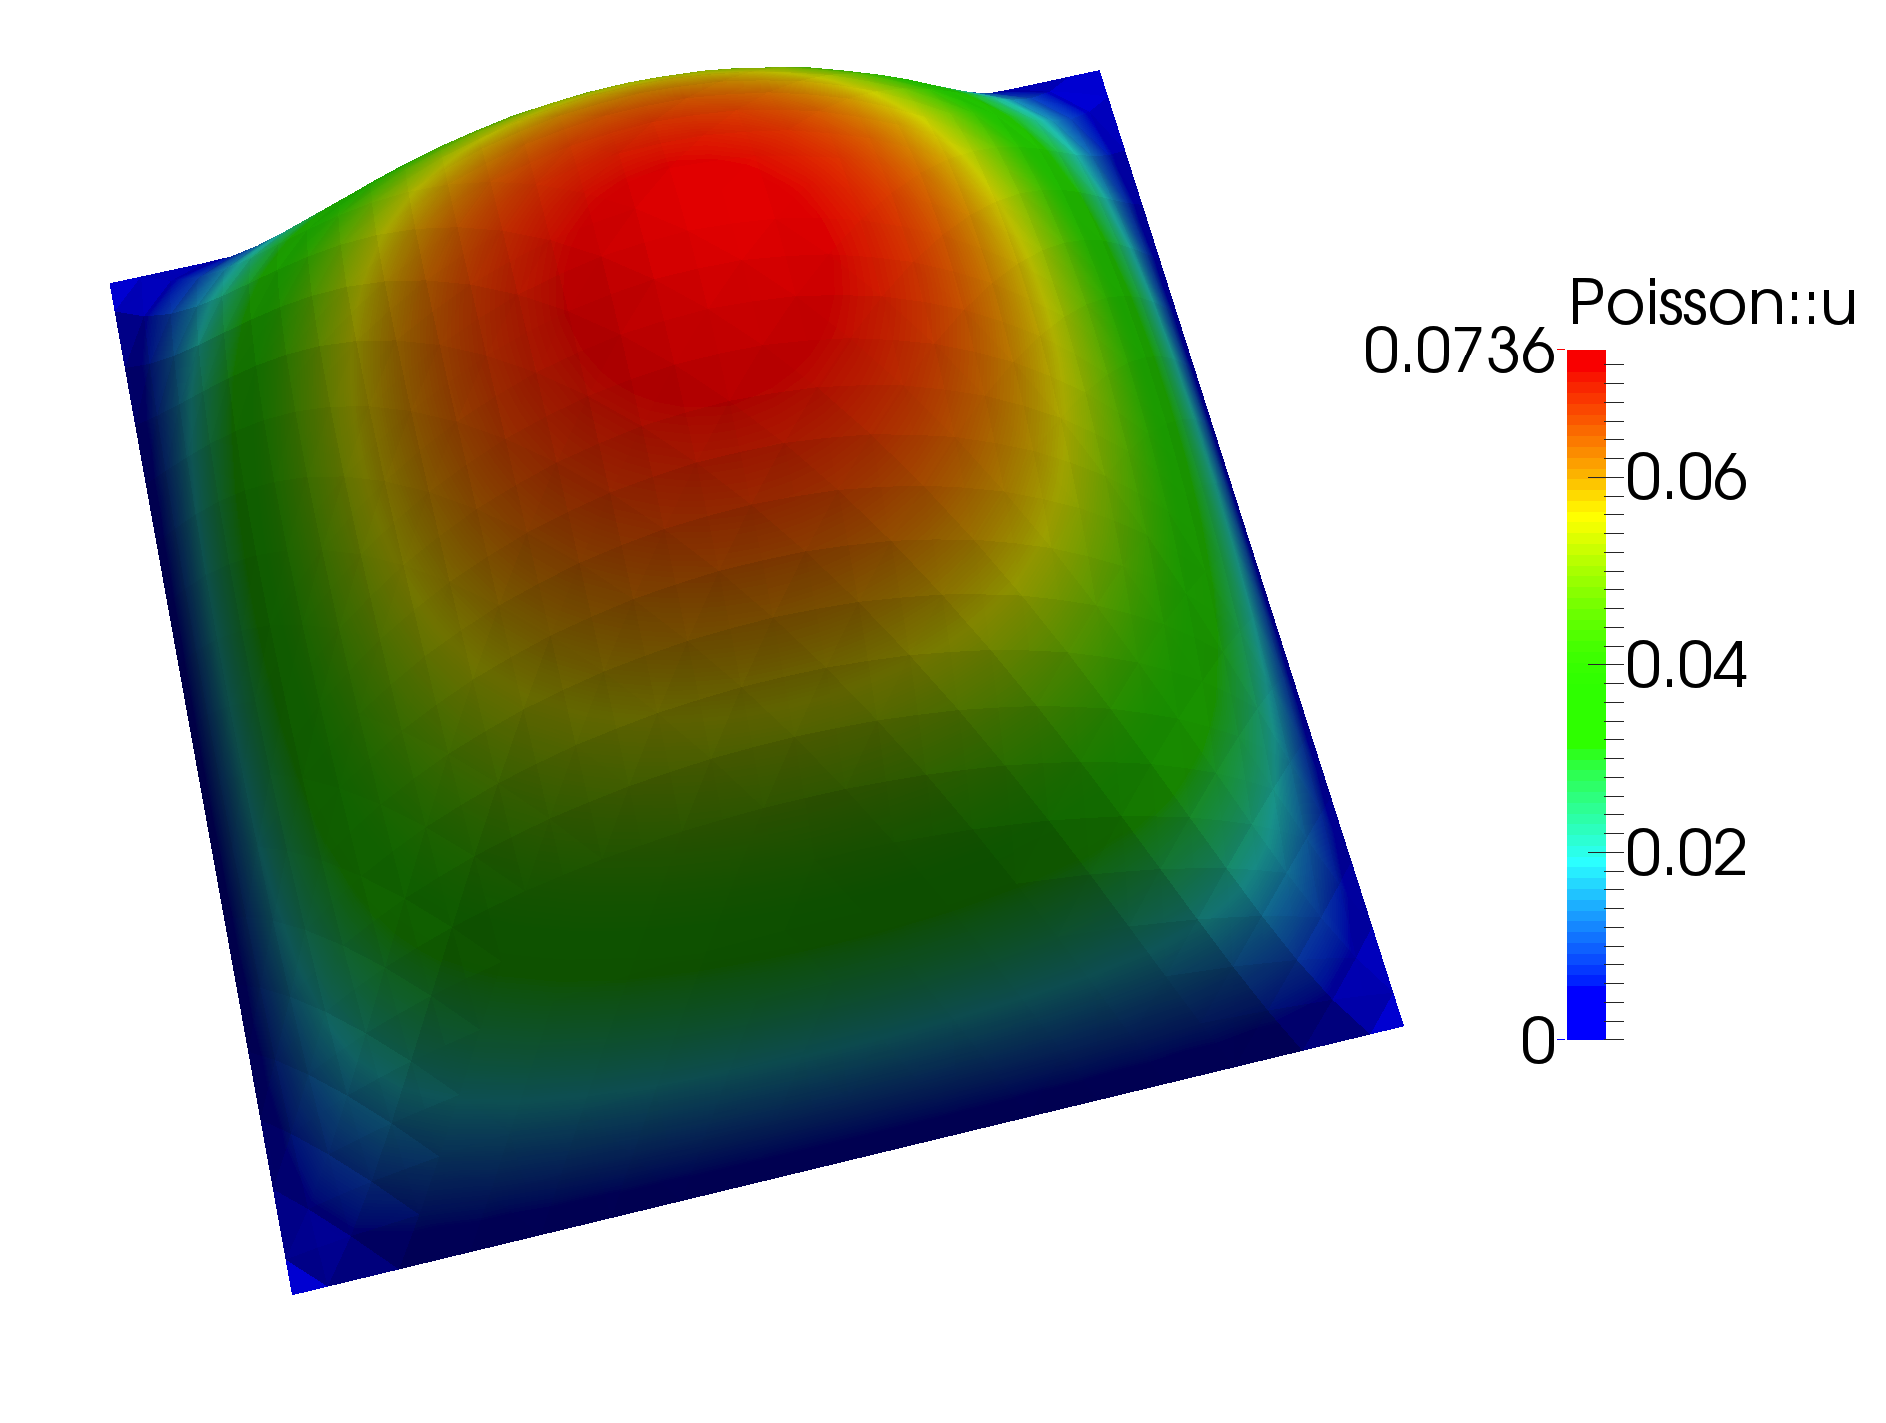
\includegraphics[width=.9\textwidth]{figures/poisson_simple.png}
  \caption{\protect\small The FEM solution of poisson's equation on the unit square
    with unit forcing and homogeneous dirichlet boundary conditions.
    This version solves the problem using piecewise linear elements P1
    on a $32\times 32$ crossed triangular mesh. The mesh can be seen
    in the facets of the solution.}
  \label{fig:simple_poisson}
\end{figure}



  
%\lstinline[style=Bash]´$ tfbuild <filename>.tfml´.




\section{Themes and Variations}
\label{sec:themes-variations}

\subsection{Manufactured Solutions}
\label{sec:manuf-solut}

\subsection{Changing Elements}
\label{sec:changing-elements}

\subsection{Changing Meshes}
\label{sec:changing-meshes}

\subsection{Changing Solvers}
\label{sec:changing-solvers}



\end{document}


